\documentclass{beamer}
\usetheme[faculty=phil, microtype, university = auth]{fibeamer}\usepackage[utf8]{inputenc}
\usepackage[english]{babel}
\usepackage{tikz}      % Diagrams
\usepackage{amsmath, amssymb}
\usepackage{url}       % `\url`s
\usepackage{listings}

\frenchspacing
\begin{document}

\begin{frame}{git}
  \begin{itemize}
  \item Created by Linus Torvalds for managing the development of
    the Linux kernel (> 18 millions line of code)
  \item It is a software for \alert{version control} focused on developing code
    with other people
  \end{itemize}
\end{frame}

\begin{frame}{git}
  \framesubtitle{For a physicist}%
  \begin{itemize}
  \item Convenient way to backup personal scripts, reports, programs
  \item Convenient way to share them
  \item Convenient way to write collaborative code and papers
  \item (Forget about Dropbox's and Drive's, duplicate files)
  \end{itemize}
\end{frame}

\begin{frame}{git}
  \framesubtitle{Basics}%
  \begin{itemize}
  \item git works in \alert{repositories}, not necessary online
  \item A repo contains all the history of a project and it is update
    only when the coder wants with only what he wants
  \item The act of updating a repo is called \alert{commit}
  \item The act of choosing what to commit is called \alert{adding}
  \item Commits are incremental (no need to save a whole file if only one
    line is changed, only the diff is saved) and usually are submitted with
    logs that explain the changes (\alert{self documentation})
  \end{itemize}
\end{frame}

\begin{frame}{git}
  \framesubtitle{Basics}%
  \begin{itemize}
  \item Two repos can be synchronized, if one of them is online this provides a
    way to perform a backup
  \item The act of updating an online repo with a local one is called \alert{pushing}
  \item The act of updating a local repo with an online one is called \alert{pulling}
  \item GitHub, GitLab, Bitbucket offer free online repos
  \end{itemize}
\end{frame}

\begin{frame}{git workflow}
  \centering
  \includegraphics[width=8cm]{images/Github.png}

  Example: Fred develops a program and push it to GitHub,
  Dave and Lisa pull it, Dave add a feature and push to GitHub,
  Fred and Lisa can pull the new version and have on their laptop
  the latest release
\end{frame}

\begin{frame}{git}
  \framesubtitle{Basics}%
  \begin{itemize}
  \item A single repo can have many \alert{branches} where code is developed independently, for example one branch for every developer or one
    for every version
  \item Branches can be \alert{merged}
  \item If there are no conflicts the merge proceeds automatically
  \item If there are conflicts someone has to review them manually
  \item On online repos it is possible to \alert{fork} other's repos and work on them and then ask for merging with the master one. This is done with a \alert{pull request} (the same when merging two branches)
  \end{itemize}
\end{frame}

\begin{frame}{git workflow}
  \centering
  \includegraphics[width=8cm]{images/workflow.png}

  \href{https://github.com/lcm-unimi/umanager/network}{Example}
\end{frame}

\begin{frame}[fragile]{Git for lazy physicists}
  % \framesubtitle{The law of big numbers and the central
  % limit theorem}%
  \begin{tikzpicture}[overlay,remember picture]
    \node[anchor=south east,xshift=-40pt,yshift=50pt]
    at (current page.south east) {
      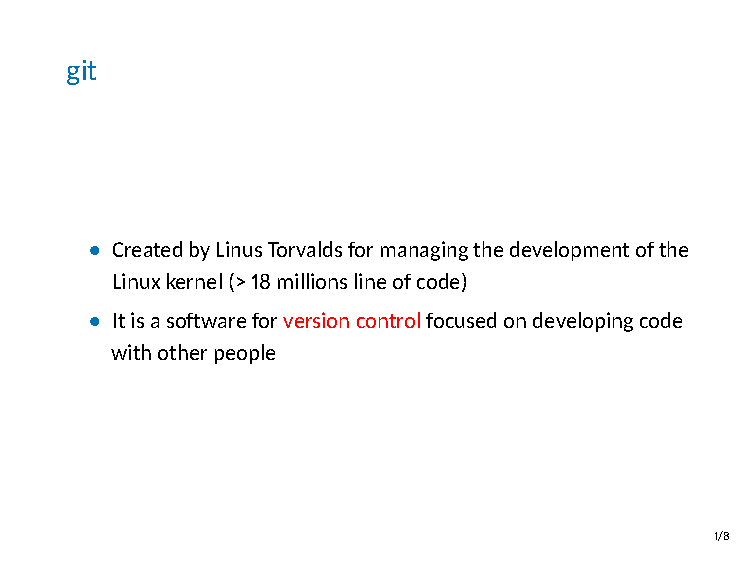
\includegraphics[width=45mm]{images/git.png}
    };
  \end{tikzpicture}%
\verb|$ git add files| \\
\verb|$ git commit| \\
\verb|$ git push origin master|
\end{frame}

\end{document}

%%% Local Variables:
%%% mode: latex
%%% TeX-master: t
%%% End:

%%% Local Variables:
%%% mode: latex
%%% TeX-master: t
%%% End:
